%\documentclass[a4paper,twoside,10pt,openright]{report}%Dokumentenklasse 
\usepackage{graphicx} %Compiler

\usepackage{dsfont}

%%%% Schrift und Kodierung %%%%
	\usepackage[T1]{fontenc} %Zeichensatzkodierung von 7bit auf 8bit 
	\usepackage[utf8]{inputenc} %Zeichensatzkodierung Unicode bzw. UTF8
	\usepackage{lmodern} %Vektorschrift
	%\RequirePackage[english,spanish,es-nolayout]{babel}
	\usepackage[english]{babel}
	\usepackage{textcomp}
	\usepackage{lmodern}
	\usepackage{url}
	\usepackage[bookmarksnumbered=true]{hyperref}
    \graphicspath{{figures/}}	
	
%%% COLORS %%%
\newcommand{\hl}[1]{
   \textcolor{MidnightBlue!90!black}{#1} 
}

\usepackage{pifont}% http://ctan.org/pkg/pifont
\newcommand{\cmark}{\ding{51}}%
\newcommand{\xmark}{\ding{55}}%

\usepackage{stackrel}

\usepackage{feynmp}

\usepackage{amsthm}
\newtheorem{definition}{Definition}
\newtheorem{proposition}{Proposition}
	
%%%% Fancy Header %%%
\usepackage{fancyhdr}
\usepackage[dvipsnames]{xcolor}
\usepackage{tikz} 
\usepackage{pgfplots}
%\usepackage{pgf-pie}

\usetikzlibrary{arrows}
\usetikzlibrary{shapes.geometric, arrows}

\definecolor{mycolor}{rgb}{0.45,0.45,0.45}% dark grey

\newcommand{\mcD}{\mathcal{D}}
\newcommand{\mcL}{\mathcal{L}}
\newcommand{\dth}{\Delta_{\text{th/sys}}}
\newcommand{\dst}{\Delta_{\text{stat}}}
\newcommand{\dsy}{\Delta_{\text{syst}}}
\newcommand{\sthsy}{\sigma_{\text{th/sys}}}
\newcommand{\sth}{\sigma_{\text{th}}}
\newcommand{\sst}{\sigma_{\text{stat}}}
\newcommand{\ssy}{\sigma_{\text{syst}}}

\newcommand{\Langle}{\big\langle}
\newcommand{\Rangle}{\big\rangle} 
 
\fancyhf{}
\fancyhead[LE]{\sffamily\color{mycolor}\nouppercase{\leftmark}} % left even, right odd
\fancyhead[RO]{\sffamily\color{mycolor}\nouppercase{\rightmark}} % left even, right odd
\fancyfoot[CE,CO]{\sffamily\color{mycolor}\nouppercase{\thepage}} % center even, center odd
\renewcommand{\headrule}{{\color{mycolor}%
\hrule width\headwidth height\headrulewidth \vskip-\headrulewidth}}
\renewcommand{\headrulewidth}{0.5pt}

\fancypagestyle{plain}{%
    \fancyhf{}%
    \fancyfoot[CE,CO]{ { \sffamily\color{mycolor}{\thepage} } }
	\renewcommand{\headrulewidth}{0.0pt}
}

%\fancypagestyle{fancy}{%
%   \fancyhf{}
%	\fancyhead[LE,RO]{\sffamily\color{mycolor}\nouppercase{\leftmark}} % left even, right odd
%	\fancyfoot[CE,CO]{\sffamily\color{mycolor}\nouppercase{\thepage}} % center even, center odd
%	\renewcommand{\headrule}{{\color{mycolor}%
%	\hrule width\headwidth height\headrulewidth \vskip-\headrulewidth}}
%	\renewcommand{\headrulewidth}{0.5pt}
%}


%%% Customize titles %%%%
\usepackage[ ]{titlesec}  %
\usepackage{etoolbox}
\makeatletter
\patchcmd{\ttlh@hang}{\parindent\z@}{\parindent\z@\leavevmode}{}{}
\patchcmd{\ttlh@hang}{\noindent}{}{}{}
\makeatother
%\titleformat{\chapter}[display]
%  { \normalsize \huge  \color{black}}%
%  {\flushright \normalsize \color{mycolor} \MakeUppercase %
%  {\sffamily \chaptertitlename } \hspace{1 ex}%
%  { \fontsize{60}{60}\selectfont \color{mycolor} \sffamily  \thechapter }}%
%  {10 pt}%
%  {\sffamily \huge \color{mycolor}\bfseries}
%\newcommand\mychapformat[1]{\parbox[t]{\dimexpr\textwidth-3em\relax}{\raggedleft#1}}
\titleformat{\chapter}[hang]{\Huge\bfseries\color{mycolor}\sffamily}% the number
	{\thechapter\hspace{20pt}\textcolor{mycolor}{|}\hspace{20pt}}%
	{0pt}{\Huge\bfseries\color{mycolor}\sffamily}% the title
\titleformat*{\section}{\sffamily\LARGE\color{mycolor}}
\titleformat*{\subsection}{\sffamily\Large\color{mycolor}}
\titleformat*{\subsubsection}{\sffamily\large\color{mycolor}}
\titleformat*{\paragraph}{\sffamily\large\bfseries\color{mycolor}}



	
%%%% Mathepakete %%%%
	\usepackage{array}
	\usepackage{calc}
	\usepackage{amsmath}
	\usepackage[intlimits]{empheq}
	\usepackage{amssymb,mathrsfs}
	\usepackage{theorem}
	\usepackage{slashed}
	\usepackage{feynmp-auto}

%%%% Sonstiges %%%%
	%\usepackage{subcaption}
	\expandafter\def\csname ver@subfig.sty\endcsname{}
	\usepackage{subfig} %Ermöglicht subfloats, also mehrere Tabellen/Bilder in einer Umgebung
	\usepackage{float} %Setzt mit [H] Figuren genau dort hin, wo sie im Text auftauchen
	\usepackage{booktabs} %Andere Tabellen
	\usepackage{gensymb}
	\usepackage{extarrows}%lange Pfeile
%	\usepackage{pst-pdf}	
	\usepackage{wasysym} %Symbolpaket
	\usepackage{multirow} %Ein Wert für mehrere Zeilen oder Spalten von Tabellen. Verwendung \multirow{#AnzahlZeilen}{*}{Name} bzw. analog \multicolumn{}{}{}
	\usepackage{rotating} %ermöglicht Schiefe Schrift
	%\usepackage{ziffer} %Deutsche Zahlen (Komma als Dezimalstelle im Mathemodus!)
	\usepackage{nicefrac} %Im Text schöne Brüche
	\usepackage[inner=3cm, outer=2.4cm, top=3cm]{geometry} %Passt Seitenränder an (left, right, top, bottom, width, height, textwidth, textheight)
	\usepackage{scrhack} %Verbessert angeblich LaTeX-Pakete
	\usepackage{numprint} %ROOT-Zahlen in deutsches zahlenformat übertragen. Syntax: \numprint[kg]{1.234e56} wird zu 1,234 * 10^56 kg
	\usepackage{cite}
	\usepackage{placeins}
	\usepackage{changepage}
	%\hyphenation{con-fine-ment}
	
%%%% spezielle Formatierungen %%%%
	\setlength{\emergencystretch}{25pt} %verhindert das Herausragen von Wörtern übers Zeilenende
	\setlength{\parindent}{0pt} %Kein Einschub bei neuem Absatz
	\setlength{\parskip}{2pt plus 1pt} %Erhöht Abstand zwischen Absätzen (um 1pt flexibel bei Seitenumbrüchen)
	
	%%%% Dokument-Variablen %%%%
\date{\today}

%%%% Eigene Befehle %%%%
\DeclareGraphicsRule{*}{mps}{*}{}
	\newcommand{\mE}[1]{\,\mathrm{#1}} %Einheiten im Mathemodus
	\renewcommand{\sl}[1]{\slashed{#1}} %Feynman-Slash
	\newcommand{\dummyImage}[2]{  %Erzeugt eine Umgebung wie includegraphics
		\frame{\mbox{\rule{0pt}{#2}	Bild fehlt  noch \rule{#1}{0pt}}}
	}
	\renewcommand{\i}{\mathrm{i}} %Imaginäre Einheit
%	\renewcommand{\vec}[1]{\textbf{#1}} %Fette Vektoren
	\newcommand{\bc}{\begin{center}}
	\newcommand{\ec}{\end{center}}

\newcommand{\matM}{\mathcal{M}}
\newcommand{\matH}{\mathcal{H}}
\newcommand{\matS}{\mathcal{S}}
\newcommand{\matU}{\mathcal{U}}
\newcommand{\matUL}{\mathcal{U}_L}
\newcommand{\matUR}{\mathcal{U}_R}

%%% center all the figures and tables
\makeatletter
\g@addto@macro\@floatboxreset\centering
\makeatother

%% maximal number of floating environments on each page 
\setlength{\floatsep}{0pt}
\setcounter{topnumber}{1}
\setcounter{bottomnumber}{1}
\setcounter{totalnumber}{1}
\renewcommand{\topfraction}{1.0}
\renewcommand{\bottomfraction}{1.0}
\renewcommand{\textfraction}{0.0}
\renewcommand{\thefootnote}{\fnsymbol{footnote}}

\def\tablename{Table}
\def\figurename{Figure}

\newcommand{\newparagraph}{\par\bigskip\noindent}
\newcommand{\toolfont}[1]{\texttt{#1}}
\newcommand{\ord}{\ensuremath{\mathcal{O}}}
\newcommand{\ope}[1]{\ensuremath{\mathcal{O}_{#1}}}
\newcommand{\largex}{\ensuremath{\large \boldsymbol{\times}}}
\newcommand{\brlargex}{\ensuremath{\large (\boldsymbol{\times})}}
\newcommand{\mheavy}{\ensuremath{M}}

\newcommand{\lag}{\ensuremath{\mathcal{L}}}
\newcommand{\mat}{\ensuremath{\mathcal{M}}}
\newcommand{\delx}{\ensuremath{\Delta}}
\newcommand{\data}{\ensuremath{\mathcal{D}}}
\newcommand{\jump}{\vspace{0.3cm}}
\newcommand{\bsg}{\ensuremath{\mathcal{B}(b \to s \gamma)}}
\newcommand{\rself}{\ensuremath{\hat{\Sigma}}}
\newcommand{\retildehat}{\ensuremath{\mbox{Re}\hat{\Sigma}}}
\newcommand{\retilde}{\ensuremath{\mbox{Re}\,\Sigma}}
\newcommand{\dweaksing}{\ensuremath{\delta_{\text{weak}}^{\text{sing}}}}
\newcommand{\dweak}{\ensuremath{\delta_{\text{weak}}}}
\newcommand{\newtext}[1]{\textcolor{red}{#1}}
\newcommand{\suit}{\textcolor{blue}{$\spadesuit$}}
\newcommand{\neutn}{\ensuremath{\tilde{\chi}^0_n}}
\newcommand{\gluino}{\ensuremath{\tilde{g}}}
\newcommand{\squark}{\ensuremath{\tilde{q}}}
\newcommand{\met}{\ensuremath{\slashed{E}_T}}
\newcommand{\nqsq}{\ensuremath{\tilde{\chi}\,\tilde{q}\,q}}
\newcommand{\msbar}{\ensuremath{\overline{MS}}}
\newcommand{\sw}{\ensuremath{s_w}}
\newcommand{\swd}{\ensuremath{s^2_w}}
\newcommand{\cw}{\ensuremath{c_w}}
\newcommand{\cwd}{\ensuremath{c^2_w}}
\newcommand{\myrbox}[1]{\parbox{4.0cm}{#1}}

\usepackage{xspace}
\newcommand{\brinv}{\ensuremath{BR_{\text{inv}}}\xspace}
\newcommand{\vegas}{\textsc{Vegas}\xspace}
\newcommand{\madgraph}{\textsc{Madgraph}\xspace}
\newcommand{\geant}{\textsc{Geant4}\xspace}
\newcommand{\pythia}{\textsc{Pythia}8\xspace}
\newcommand{\fastjet}{\textsc{FastJet}\xspace}
\newcommand{\delphes}{\textsc{Delphes}\xspace}
\newcommand{\sherpa}{\textsc{Sherpa}\xspace}
\newcommand{\sklearn}{\textsc{scikit-learn}\xspace}
\newcommand{\keras}{\textsc{Keras}\xspace}
\newcommand{\tensorflow}{\textsc{TensorFlow}\xspace}
\newcommand{\pytorch}{\textsc{PyTorch}\xspace}
\newcommand{\theano}{\textsc{Theano}\xspace}
\newcommand{\adam}{\textsc{Adam}\xspace}

\newcommand{\psib}{\overline{\psi}}
\newcommand{\bpm}{\begin{pmatrix}}
\newcommand{\epm}{\end{pmatrix}}

\newcommand{\p}{\partial}
\newcommand{\br}{\text{BR}}
\newcommand{\qqquad}{\qquad \qquad}
\newcommand{\qqqquad}{\qquad \qquad \qquad}

\newcommand{\matx}{|\mathcal{M}|^2}
\newcommand{\really}{\stackrel{!}{=}}
\newcommand{\SFitter}{\textsc{SFitter} }

% units of measure
\newcommand{\mev}{{\ensuremath\rm MeV}}
\newcommand{\gev}{{\ensuremath\rm GeV}}
\newcommand{\tev}{{\ensuremath\rm TeV}}
\newcommand{\fb}{{\ensuremath\rm fb}}
\newcommand{\ab}{{\ensuremath\rm ab}}
\newcommand{\pb}{{\ensuremath\rm pb}}
\newcommand{\sign}{{\ensuremath\rm sign}}
\newcommand{\iab}{\text{ab}^{-1}}
\newcommand{\ifb}{{\ensuremath\rm fb^{-1}}}
\newcommand{\ipb}{{\ensuremath\rm pb^{-1}}}

% really great macro by Chris Lester
\def\slashchar#1{\setbox0=\hbox{$#1$}           % set a box for #1
   \dimen0=\wd0                                 % and get its size
   \setbox1=\hbox{/} \dimen1=\wd1               % get size of /
   \ifdim\dimen0>\dimen1                        % #1 is bigger
      \rlap{\hbox to \dimen0{\hfil/\hfil}}      % so center / in box
      #1                                        % and print #1
   \else                                        % / is bigger
      \rlap{\hbox to \dimen1{\hfil$#1$\hfil}}   % so center #1
      /                                         % and print /
   \fi}
\newcommand{\dslash}{\slashchar{\partial}}
\newcommand{\Dslash}{\slashchar{D}}

\def\eg{{e.g.}\ }
\def\ie{{i.e.}\ }
%\def\etal{{\sl et al} \,}
%\DeclareMathOperator{\tr}{Tr}
\newcommand{\pbp}{\ensuremath{H^\dagger\,H}}
\DeclareMathOperator{\tr}{Tr}
\newcommand{\Dfb}{\mbox{$\raisebox{2mm}{\boldmath ${}^\leftrightarrow$}\hspace{-4mm} D$}}
\newcommand{\Dfba}{\mbox{$\raisebox{2mm}{\boldmath ${}^\leftrightarrow$}\hspace{-4mm} D^a$}}
\newcommand{\overbar}[1]{\mkern 1.5mu\overline{\mkern-1.5mu#1\mkern-1.5mu}\mkern 1.5mu}
\let\vec\mathbf % vectors in bold
\renewcommand{\d}{\text{d}}


%\pagestyle{fancy}
%\graphicspath{{../figures/}}	
%\begin{document}

\chapter{Introduction}\label{chap:introduction}
\enlargethispage{2ex}
\vspace*{-2pt}

The research program carried over at the Large Hadron Collider (LHC) relies on vast amount of synthetic data to perform hypothesis tests~\cite{Apostolakis:2308666, Aarrestad:2729448, Calafiura:2729668, ATL-SOFT-PUB-2018-002}. Simulations of parton level interactions and the subsequent processes of parton showering and hadronization, as well as the simulation of detector effects, are traditionally performed with Monte Carlo methods. These methods are built using first-principles, in the sense that they are expected to describe the corresponding physical system to the best of our knowledge, being that a detector or a quantum field theory. 
However, precision and interpretability don't come for free, and a major shortcoming of these methods lies in their computational efficiency. In fact, Monte Carlo simulations takes the biggest share of computational resources of collaborations working at the LHC, with detector simulations being the biggest contributors~\cite{Calafiura:2729668}. As a notable example, the time needed to fully simulate a detector response with \geant~\cite{AGOSTINELLI2003250} is of the order of minutes.
If we give up on the idea of simulating a physical system from first principles, we can reformulate the problem entirely as a sampling task: a detector image may be for instance regarded as a sample from an hypothetical distribution $p_{detector}$ defined on some high-dimensional space. The same idea may be applied to other stages of the simulation pipeline, such as the simulation of parton level events, or parton showers.
If samples drawn from such a distribution can be used as a surrogate for first principle simulations, massive gains in computational time are theoretically possible, hence the recent interest in the potential of deep generative models for particle physics (see \href{https://iml-wg.github.io/HEPML-LivingReview}{HEPML-LivingReview} to get the full picture).

Deep generative models are a natural tool for supporting  (or replacing) traditional Monte Carlo simulations, as they have the necessary expressive power to accurately reproduce complex, high-dimensional and multi-modal distributions. Furthermore, the field of high energy physics doesn't suffer from a typical bottleneck of applied deep learning, where clean, labelled natural images, texts, or biomedical data, can be expensive to obtain or be protected by privacy laws. Conversely, truly large, particle physics datasets are either publicly available or can be in most cases cheaply generated.

The potential of deep generative models goes beyond the production of synthetic data, and, depending on the particular framework, they can solve a variety of tasks such as classification or anomaly detection. In this thesis, we introduce a novel method, whereby a deep generative model is employed to unfold detector effects down to the parton level.

In the remaining part of Chap.~\ref{chap:introduction} we introduce the two main topics of the thesis, generative models and the unfolding problem. Chap.~\ref{chap:unfolding} - \ref{chap:lsr} are built upon Ref.~\cite{cond_gan, Bellagente:2020piv, Bellagente:2021yyh, LSR}: first we illustrate a method for unfolding of detector effects based on deep generative models, then we address key technical aspects for a realistic use in LHC analysis, namely how to define uncertainties over a deep generative model's output, and how to handle topology obstructions induced by parton level cuts. We conclude with a summary of the main results and of possible future directions.

\section{Generative models}\label{sec:gmm}
Given data instances $\mathcal{X} = \{ x_1, \ldots , x_N \}$, a generative model is a probabilistic model of $p(x)$, i.e. of the underlying probability density from which $\mathcal{X}$ is sampled. 
In machine learning, generative modelling, or density estimation, is the unsupervised task of approximating a probability density via a parametrized function $G_{\theta}$, whose parameters $\theta$ are inferred in an automatic fashion. If $G_{\theta}$ is a good approximation of $p(x)$, new and realistic samples can be drawn from it.
Similarly, if the data comes with labels $\mathcal{Y}$, we wish to approximate the conditional probability density $p(x | y)$ with a conditional probabilistic model $G_{\theta}(x | y)$.
The underlying assumption of density estimation is that the manifold on which $\mathcal{X}$ lies can be described by a number of parameters which is lower than the dimensionality of the data itself, this way $G_{\theta}$ 
is forced to discover regularities and patterns of the input data.

As an example, given some multi-modal distribution $p(x)$, we may represent it compactly with a finite mixture
%
\begin{align}
p(x) = \sum_{k=1}^{K} \pi_{k} p_{k}(x)
\end{align}
%
with mixture weights $\pi_{k}$ constrained as
%
\begin{align}
0 \leq \pi_k \leq 1, \quad \sum_{k=1}^{K} \pi_{k} = 1.
\end{align}
%
The components $p_{k}(x)$ belong to a family of a basic distributions, e.g. Gaussians $\mathcal{N}_k(x | \mu_k, \Sigma_k)$, in which case we call the model Gaussian Mixture Model (GMM). The model's parameters $\theta = \{ \mu_k, \Sigma_k, \pi_k; ~ k = 1, \ldots, K \}$ can be inferred via Maximum Likelihood. Assuming that the points in the dataset $\mathcal{X} = \{x_1, \ldots , x_N \}$ are identically and independently distributed, the likelihood can be written in the factorized form
%
\begin{align}
p(\mathcal{X} | \theta ) = \prod_{n=1}^N p(x_n | \theta), \quad p(x_n | \theta) = \sum_{k=1}^K \pi_k \mathcal{N}_k(x_n | \mu_k, \Sigma_k),
\end{align}
%
leading to the log-likelihood
%
\begin{align}
\mathcal{L} \coloneqq \log p(\mathcal{X} | \theta ) = \sum_{n=1}^N \log \sum_{k=1}^K \pi_k \mathcal{N}_k(x_n | \mu_k, \Sigma_k).
\end{align}
%
The optimal parameters $\theta^{*}$ are those that maximize the log-likelihood, and can therefore be obtained by solving for $\theta$ the equation $\text{d} \mathcal{L} / \text{d}\theta = 0$.
As a concrete example, taking the derivative of $\mathcal{L}$ with respect to $\mu_{k}$ yelds
%
\begin{align}
\frac{\partial \mathcal{L}}{\partial \mu_k} &= \sum_{n=1}^{N} \frac{1}{p(x_n | \theta)} \frac{\partial p(x_n | \theta) }{\partial \mu_k} = \sum_{n=1}^{N} (x_n - \mu_k)^{T} \Sigma_k^{-1} \frac{\pi_k \mathcal{N}(x_n | \mu_k, \Sigma_k)}{\sum_{j=1}^{K} \pi_j N(x_n | \mu_j, \Sigma_j) } \\
&= \sum_{n=1}^{N} r_{nk} (x_n - \mu_k)^{T} \Sigma_k^{-1} .
\end{align}
%
Setting $\partial \mathcal{L} / \partial \mu_k  = 0$ we obtain
%
\begin{align}
\mu_k^{*} = \frac{1}{ \sum_{n=1}^{N} r_{nk}} \sum_{n=1}^{N} r_{nk} x_n,
\end{align}
%
where we have defined the responsibilities
%
\begin{align}
r_{nk} = \frac{\pi_k \mathcal{N}(x_n | \mu_k, \Sigma_k)}{\sum_{j=1}^{K} \pi_j N(x_n | \mu_j, \Sigma_j) }.
\end{align}
%
Similarly, it is possible to show that both $\pi_k^{*}$ and $\Sigma_k^{*}$ can also be expressed in terms of $r_{nk}$. 
As it is often the case in machine learning, there is no closed form solution to the maximization problem for $k > 1$, and we rely instead on an updating scheme which, starting from randomized values of $\theta$, iteratively finds a better approximation of $\theta^{*}$.
In the contest of GMMs, this iterative solution is called Expectation-Minimization algorithm~\cite{ExpMin1}, and can be summarized as
%
\begin{itemize}
\item
Initialize $\mu_k, \Sigma_k, \pi_k$;
\item
E-step: evaluate the responsibilities $r_{nk}$ using current parameters $\mu_k, \Sigma_k, \pi_k$;
\item
M-step: estimate the new values $\mu_k^{*}, \Sigma_k^{*}, \pi_k^{*}$ using the current responsibilities.
\end{itemize}
Each E/M-step increases the likelihood~\cite{ExpMin2}. The number of repetition and mixtures are hyperparameters.
In Fig.~\ref{fig:gmm} we show a simple example of a Gaussian mixture model used to predict the density of a 2-dimensional dataset.
%------------------------------------------------------------
\begin{figure}[t]
\centering
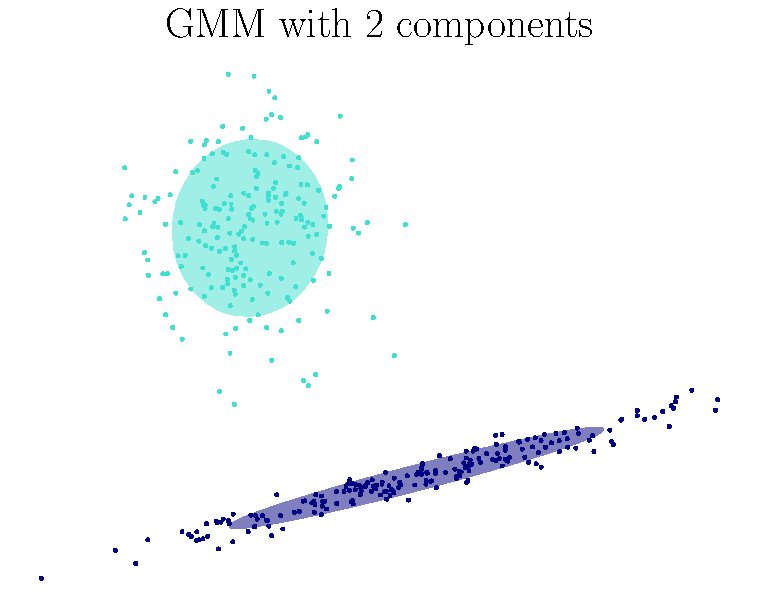
\includegraphics[page = 1, width=0.49\textwidth]{./figures/gmm}
\caption{Gaussian mixture model with two components. The equal probability surfaces are highlighted in colours.}
\label{fig:gmm}
\end{figure}
%------------------------------------------------------------

\section{Deep Generative Models}\label{sec:DGM}
We may regard the GMM as the simplest form of statistical model. Recent years have seen the advent of novel methods for generative modelling which we collectively refer to as Deep Generative Models (DGM), in complete analogy to what Deep Learning (DL) means with respect to ML. 
Before describing the most relevant forms of DGMs, and with no claim of completeness, we recall that some of the key features of DL include
\begin{itemize}
\item
models are parametrized by Neural Networks (NN) whose specific form depends on the particular task;
\item
the NN parameters are inferred via a stochastic gradient descent approach;
\item
in order to really exploit NNs, vast amount of high-fidelity data is needed for their training.
\end{itemize}
The last bullet is particularly attractive for LHC analysis, in that not only scientific collaborations such as ATLAS and CMS have already collected petabytes of data (with a lot more to come with the next upgrade of the collider), but we are also able to generate synthetic data from first principles via Monte Carlo simulations. It is therefore not surprising that DGMs have been extensively used in particle physics. Given the variety of applications and the number of papers on the topic, we refer to \href{https://github.com/iml-wg/HEPML-LivingReview}{here} for a complete overview.

Concerning the practical realisation of DGMs, the three most successful frameworks studied and employed in the literature are
\begin{itemize}
\item
Normalizing Flows (NF);
\item
Generative Adversarial Networks (GAN);
\item
Variational Autoencoders.
\end{itemize}
The first two have been extensively employed in this thesis, and will be therefore further elaborated in the following sections.

\subsubsection{Normaling Flows}\label{intro:normflow}
Normalizing Flow (NFs)~\cite{inn,coupling2,glow, nflow1,papamakarios2019normalizing,nflow_review,mller2018neural, grathwohl2018ffjord,chen2019neural} are defined in terms of a parametrized change of variable $G_{\theta}: x \rightarrow z$ between distributions
%
\begin{align}\label{eq:nf}
p_X(x) = p_Z(z) \left|\det \frac{\partial G_{\theta}(z)}{\partial z}\right|^{-1} = p_Z(\bar{G}_{\theta}(x)) \left|\det \frac{\partial \bar{G}_{\theta}(x)}{\partial x}\right|,
\end{align}
%
where $\bar{G} = G^{-1}$.
Regardless of how complicated $p_{X}(x)$ may be, if there exists a bijection $G_{\theta}$ such that $p_Z(z)$ is a simple distribution, e.g. a Gaussian $\mathcal{N}_{\mu=0, \Sigma=\mathbb{I}}$, we can draw samples from $p_{X}(x)$ via the generative pipeline
%
\begin{align}
z \sim p_Z(z) \longrightarrow x = G_{\theta}(z)  \sim p_{X}(x),
\end{align}
%
%
%------------------------------------------------------------
\begin{figure}[t]
\centering
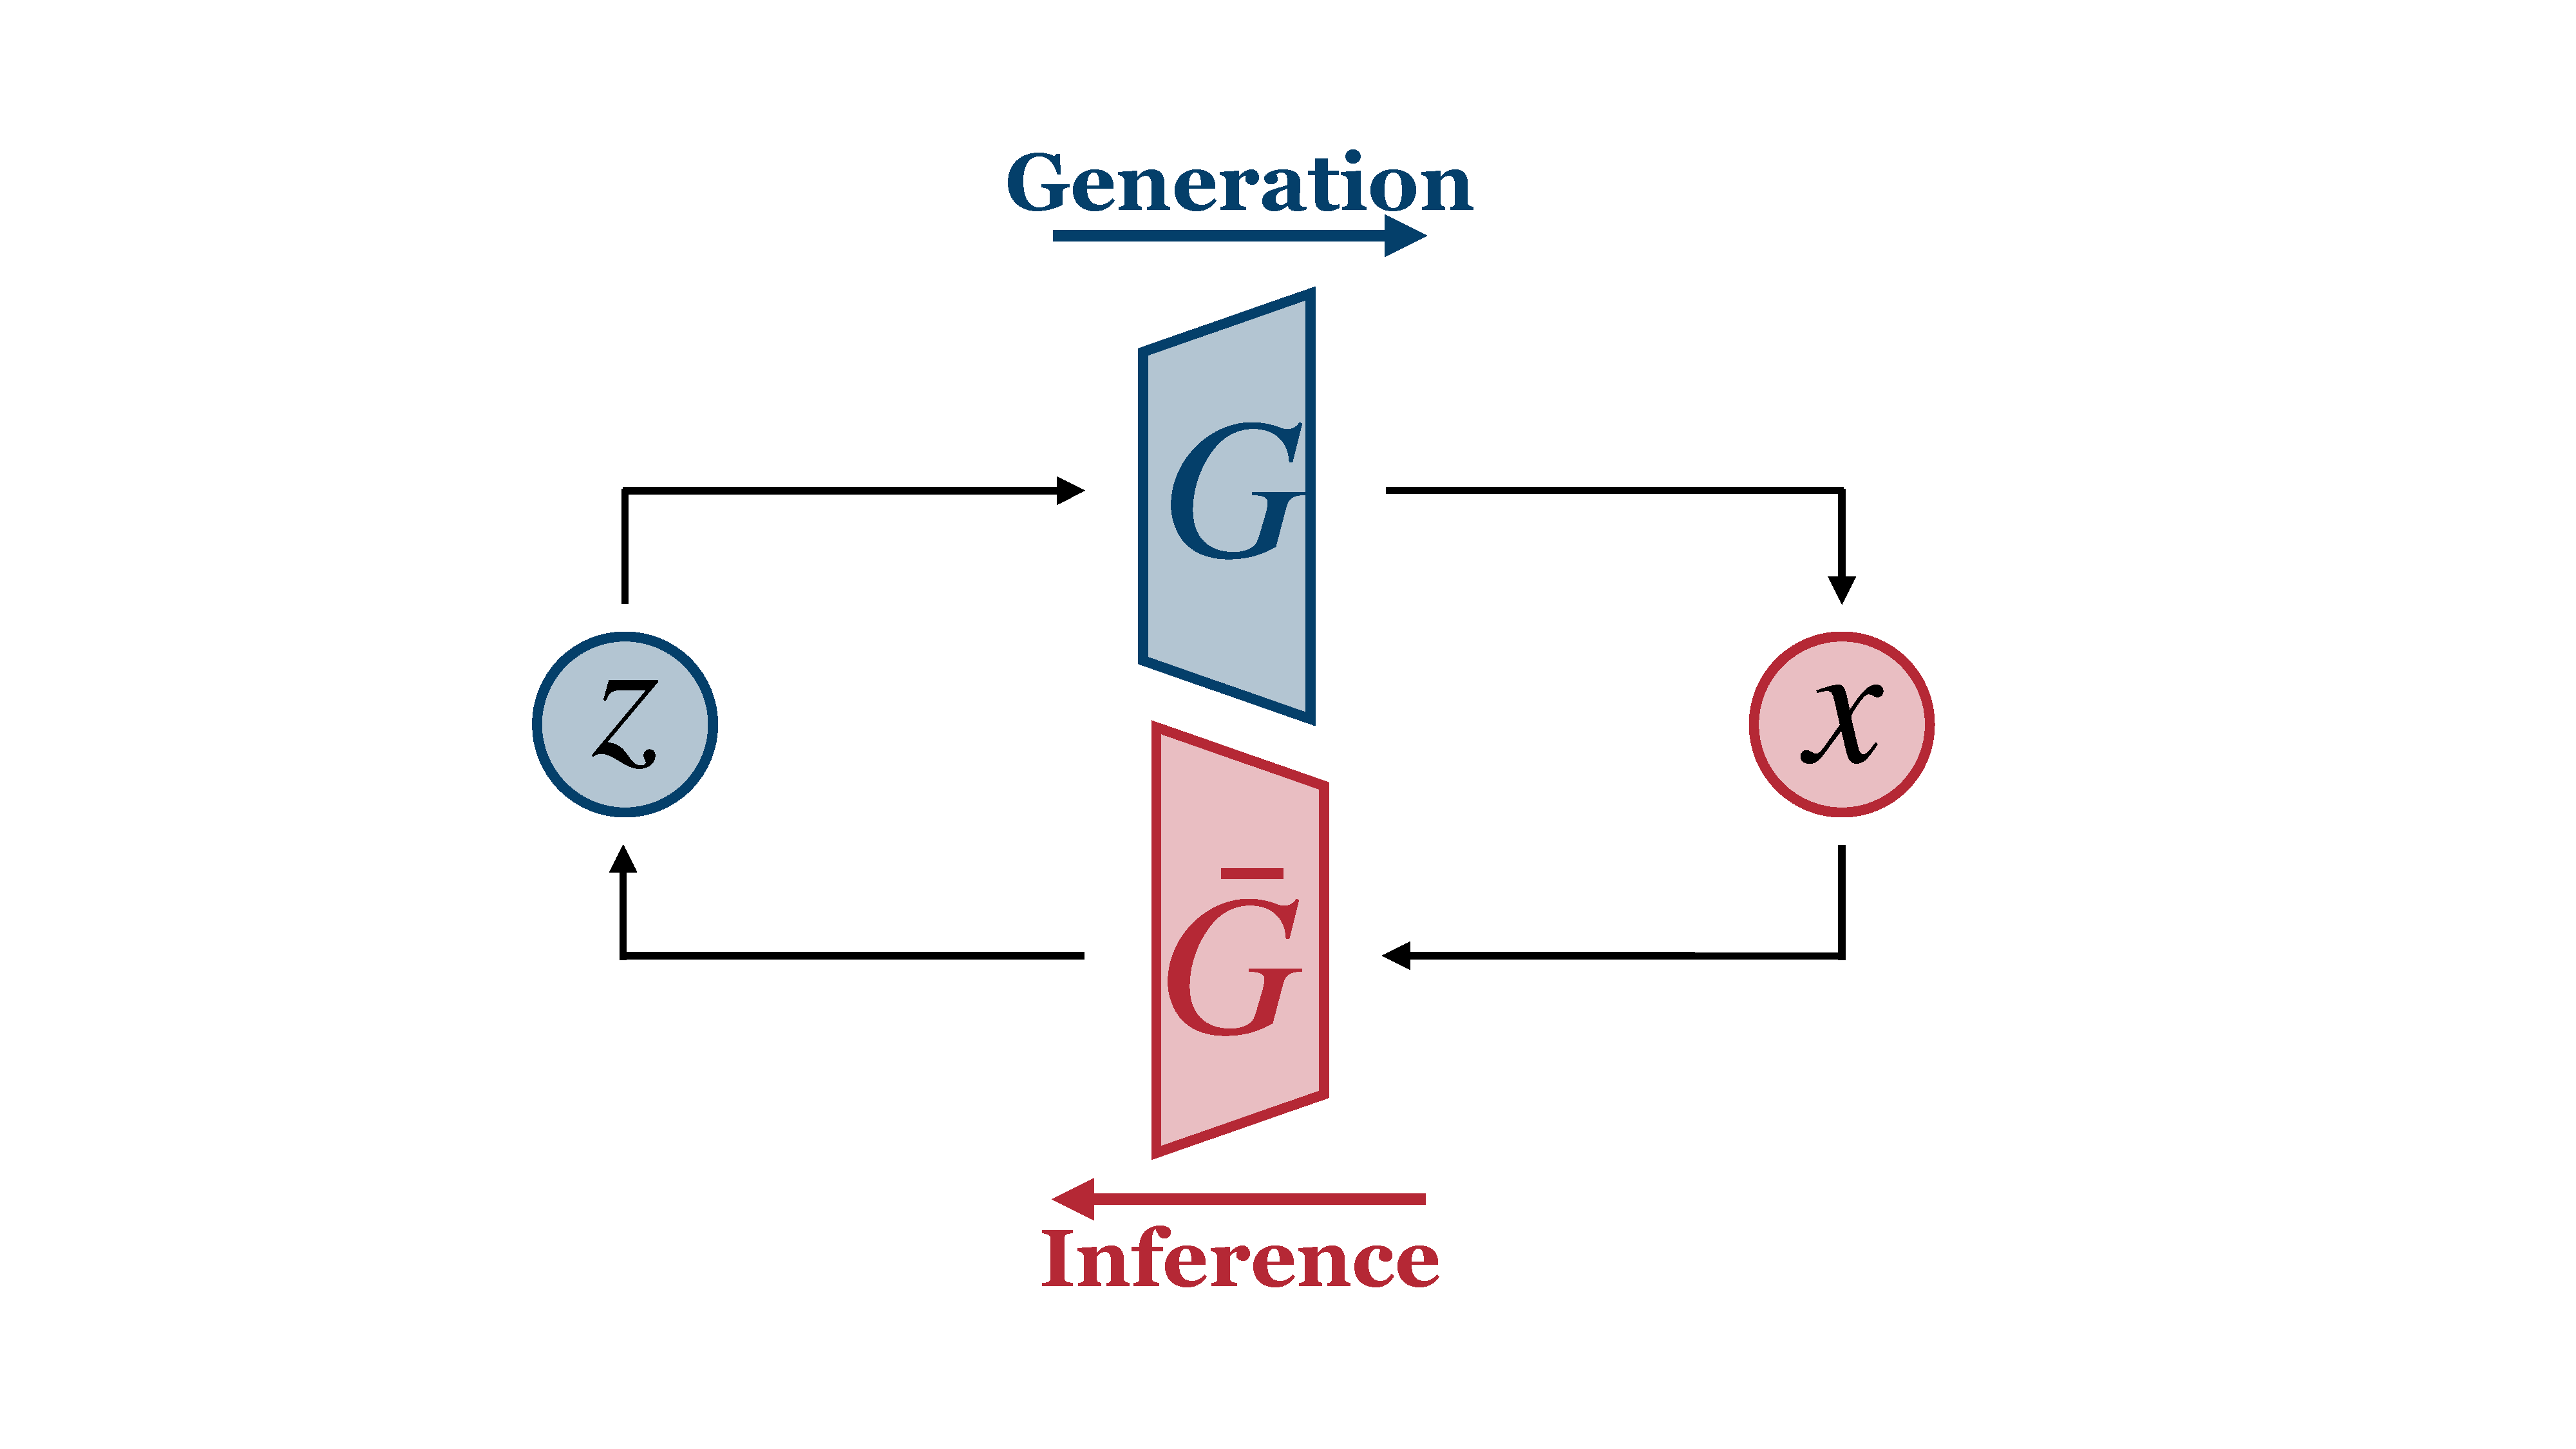
\includegraphics[page = 1, width=0.99\textwidth]{./figures/inn}
\caption{Schematic representation of a NF: a random variable $z$ sampled from a fixed, simple distribution is transformed via a map $G$ to a sample $x$ sampled from a complex target distribution. If $G$ is a bijection, and its inverse $\bar{G} = G^{-1}$ can be easily evaluated, the inverse direction can be used to train the model with Maximum Likelihood.}
\label{fig:NF}
\end{figure}
%------------------------------------------------------------
%
see Fig.~\ref{fig:NF} for a schematic representation. Similar to GMM example in Sec.~\ref{sec:gmm}, the parameters of $G_{\theta}$ can be chosen to minimize the negative log-likelihood
%
\begin{align}\label{eq:change_of_variable}
\mathcal{L} &= - \sum_{n=1}^N \log \left[ p_Z(\bar{G} _{\theta}(x_n)) \left|\det \frac{\partial \bar{G} _{\theta}(x)}{\partial x_n}\right| \right]\\
&= -\sum_{n=1}^N \log p_Z(\bar{G} _{\theta}(x_n)) + \log \left|\det \frac{\partial \bar{G} _{\theta}(x_n)}{\partial x_n}\right|\\
&= \sum_{n=1}^N \frac{(\bar{G} _{\theta}(x_n))^2}{2} - \log \left|\det \frac{\partial \bar{G} _{\theta}(x_n)}{\partial x_n}\right|
\end{align}
%
where we have used $p_{Z}(z) = \mathcal{N}_{\mu=0, \Sigma=\mathbb{I}}$ and have discarded irrelevant constant terms. 
In practice, we only need to compute $\bar{G} _{\theta}(x_n)$, the corresponding determinant of the Jacobian, and minimize the combination in the final line of Eq.~\ref{eq:change_of_variable}.

This rather straightforward blueprint hides three complications one needs to carefully address. First of all, not only $G_{\theta}$ must be a bijection, i.e. its inverse must exist, but both $G_{\theta}$ and $\bar{G} _{\theta}$ must be efficiently computable, as one is required for training and the other for generating. Finally, the map must have a tractable Jacobian. If $G_{\theta}$ is parametrized by a standard NN, such as a Multi-Layer Perceptron (MLP), none of the three properties is satisfied. These constraints restrict the class of allowed transformations, severely limiting the expressive power at our disposal, and, as a result, this research line is primarily dedicated to find the optimal trade-off between computational complexity and model expressive power. 
However, not all hope is lost, as we can build progressively more complex maps by simply stacking many simple functions, while maintaining the tractability of the Jacobian.
Given a bijection $G_{i}$ with inverse $\bar{G}_{i}$ and a cheap Jacobian, the composition
\begin{align}
G = G_{n} \cdot  G_{n-1} \ldots \cdot G_{1}
\end{align}
has inverse
\begin{align}
\bar{G} = \bar{G}_{1} \cdot   \ldots \cdot \bar{G}_{n-1} \cdot \bar{G}_{n},
\end{align}
and its determinant is the product of each individual determinant
\begin{align}
\det G = \prod_{i=1}^{N}  \det G_{i}.
\end{align}

We conclude this section with a comment motivating the study of Chap.~\ref{chap:lsr}. As already stated, invertible models are bijections, or homeomorphisms~\cite{dupont2019augmented,  huang2020augmented} (note that this is a strict equivalence, i.e. an invertible model do not approximate an homeomorphism, it is one), and as such they are by construction unable to map manifolds with different topological features, such as the number of holes and disconnected patches. In particular, if we stick to the standard formulation and only consider Gaussian latent spaces, we may only be able to represent data whose underlying manifold is compact and has genus zero. As this may be a limiting factor for the naive use of normalizing flows in particle physics, in Chap.~\ref{chap:lsr} we illustrate a possible method to account for it.

\subsubsection{Generative Adversarial Networks}\label{intro:gan}
GANs introduce a brand new paradigm for generative modelling which, unlike the previously described methods, doesn't involve computing the likelihood at all, and is therefore a form of likelihood-free machine learning. Instead, GANs rely on a two-sample test between distributions, i.e. a statistical test to determine whether or not two samples are drawn from the same distribution. This test is formulated as a differentiable objective function so that it can be minimized with stochastic gradient descent methods, in such a way that it is minimal iff the two distributions are statistically identical.
The statistical test is performed by a discriminator $D_{\phi}$ whose job is to tell apart real and fake samples. The final piece of a GAN is a generator $G_{\theta}$, a map from noise $z$ to target samples $\tilde{x}$, see Fig.~\ref{fig:gan}. In DL, both $D_{\phi}$ and $G_{\theta}$ are properly shaped NNs.
%
%------------------------------------------------------------
\begin{figure}[t]
\centering
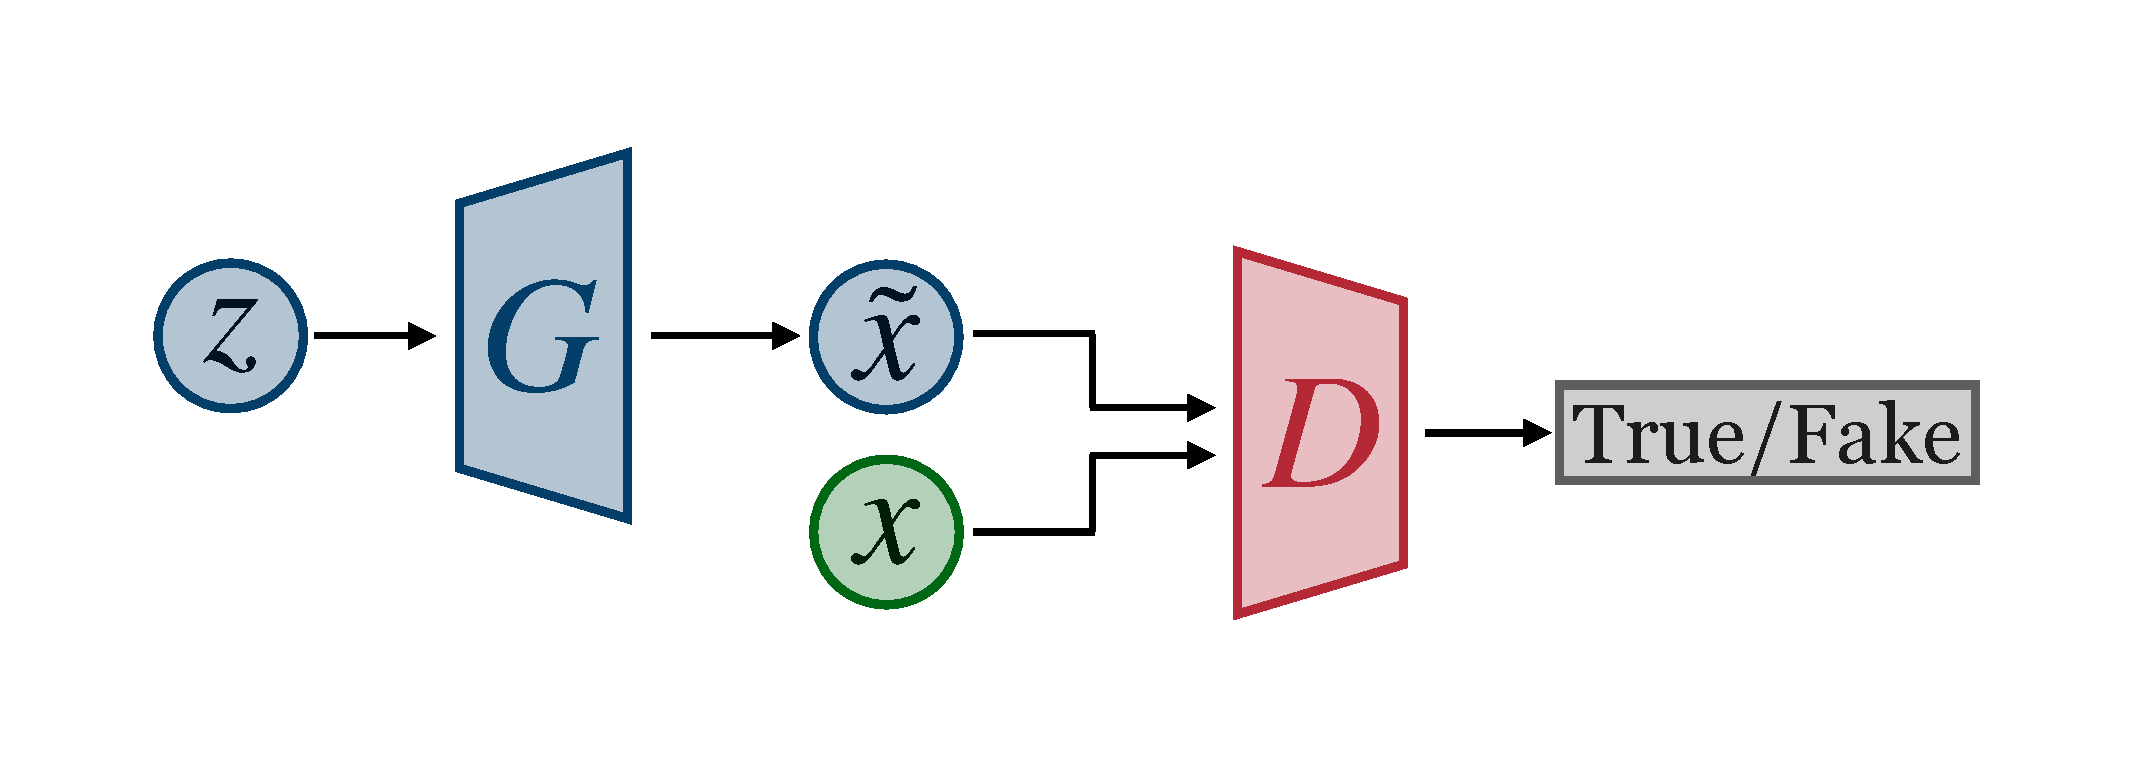
\includegraphics[page = 1, width=0.99\textwidth]{./figures/gan}
\caption{Schematic representation of a GAN: a generator $G$ deterministically maps noise $z$ to fake samples $\tilde{z}$. The discriminator $D$ is trained as a binary classifier of true versus fake data, while $G$ tries to fool it.}
\label{fig:gan}
\end{figure}
%------------------------------------------------------------
%
While many different ways to define the GAN objective have been proposed, we refer to the original formulation as it is close to the one employed in Chap.~\ref{chap:unfolding}. Formally, we consider the min-max game 
%
\begin{align}
\min_{\theta} \max_{\phi} = \mathbb{E}_{x \sim p_{X}(x)} \left[ \log D_{\phi} (x) \right] + \mathbb{E}_{z\sim p_{Z}(z)} \left[ \log \left( 1 - D_{\phi} (G_{\theta}(z) \right) \right].
\end{align}
%
For a fixed generator, this is nothing other than a binary classification task, and an optimal discriminator should output $1$ for any $x \sim p_{X}(x)$ and $0$ otherwise, which we can summarize as
%
\begin{align}
D_{\phi^{*}}(x) = \frac{p_{X}(x)}{p_{X}(x) + p_{G}(x)},
\end{align}
%
$p_{G}(x)$ being the distribution implicitly defined by the generator. 
Fixing $\phi = \phi^{*}$, the generator part of the objective is equivalent to minimizing the Jenson-Shannon divergence $JS(p_{X}, p_{G})$, with
%
\begin{align}
JS\left(p, q\right) = \frac{1}{2} \left(KL\left(p, \frac{p + q}{2}\right) + KL\left(q, \frac{p + q}{2}\right) \right),
\end{align}
%
and $KL(a, b)$ is the Kullback-Leibler divergence between $p$ and $q$. This objective has a global minimum for $p_{G} = p_{X}$.
It turns out that if the discriminator is optimal, the objective function has vanishing gradient for the generator, leading to the standard alternating training of GANs: every $k$ updates of $\phi$ we perform an update of $\theta$, $k$ being a hyperparameter.
Training a GAN is a highly non trivial task with many potential issues if extra care is not taken, notably
\begin{itemize}
\item
the optimization procedure is typically unstable and needs to be regularized;
\item
for multi-modal targets, generators can collapse to a single mode;
\item
since the objective function is not convex, there is no clear way to evaluate the model performances or to determine a stopping point.
\end{itemize}
%Plenty of empirical tips and tricks to stabilize the training of GANs are available in the literature, in the form of modified objective functions, gradient penalties, noise injection, specific optimizers and more.

An important difference between the two presented frameworks is that a GAN represents a target density only implicitly, i.e. $G_{\theta}$ is only a sampler from $p_{X}$, but can't be used to estimate its value (with the exception of low dimensional problems where kernel methods may be used to smooth a binned distribution). On the other hand, the explicit value of the density can be trivially computed with a NF from Eq.~\ref{eq:nf} if we assume a perfect map to the latent space distribution.

\section{Bayesian unfolding}

In this section we will define the fundamental ideas of unfolding following closely Ref.~\cite{DAgostini:1994fjx, dagostini2010improved}.
In any quantitative science we wish to be able to estimate the possible value of "true" parameters, directly connected to some underlying theory, given that we are only able of observing a distorted version of them in the best scenario, more realistically we will have to be satisfied with observing a different set of parameters entirely.
In particular, we are often interested in lifting the effects induced by the detectors and possible physical and theoretical backgrounds. This procedure is normally called de-convolution, and takes the name of unfolding in particle physics.

Bayesian inference is the proper framework to perform inference over unknown parameters from experimental data. A starting point for Bayesian unfolding is the discretization of the problem, in the form of binning of observable distribution of events, with each bin being treated as an independent variables.
%
%------------------------------------------------------------
\begin{figure}[t]
\centering
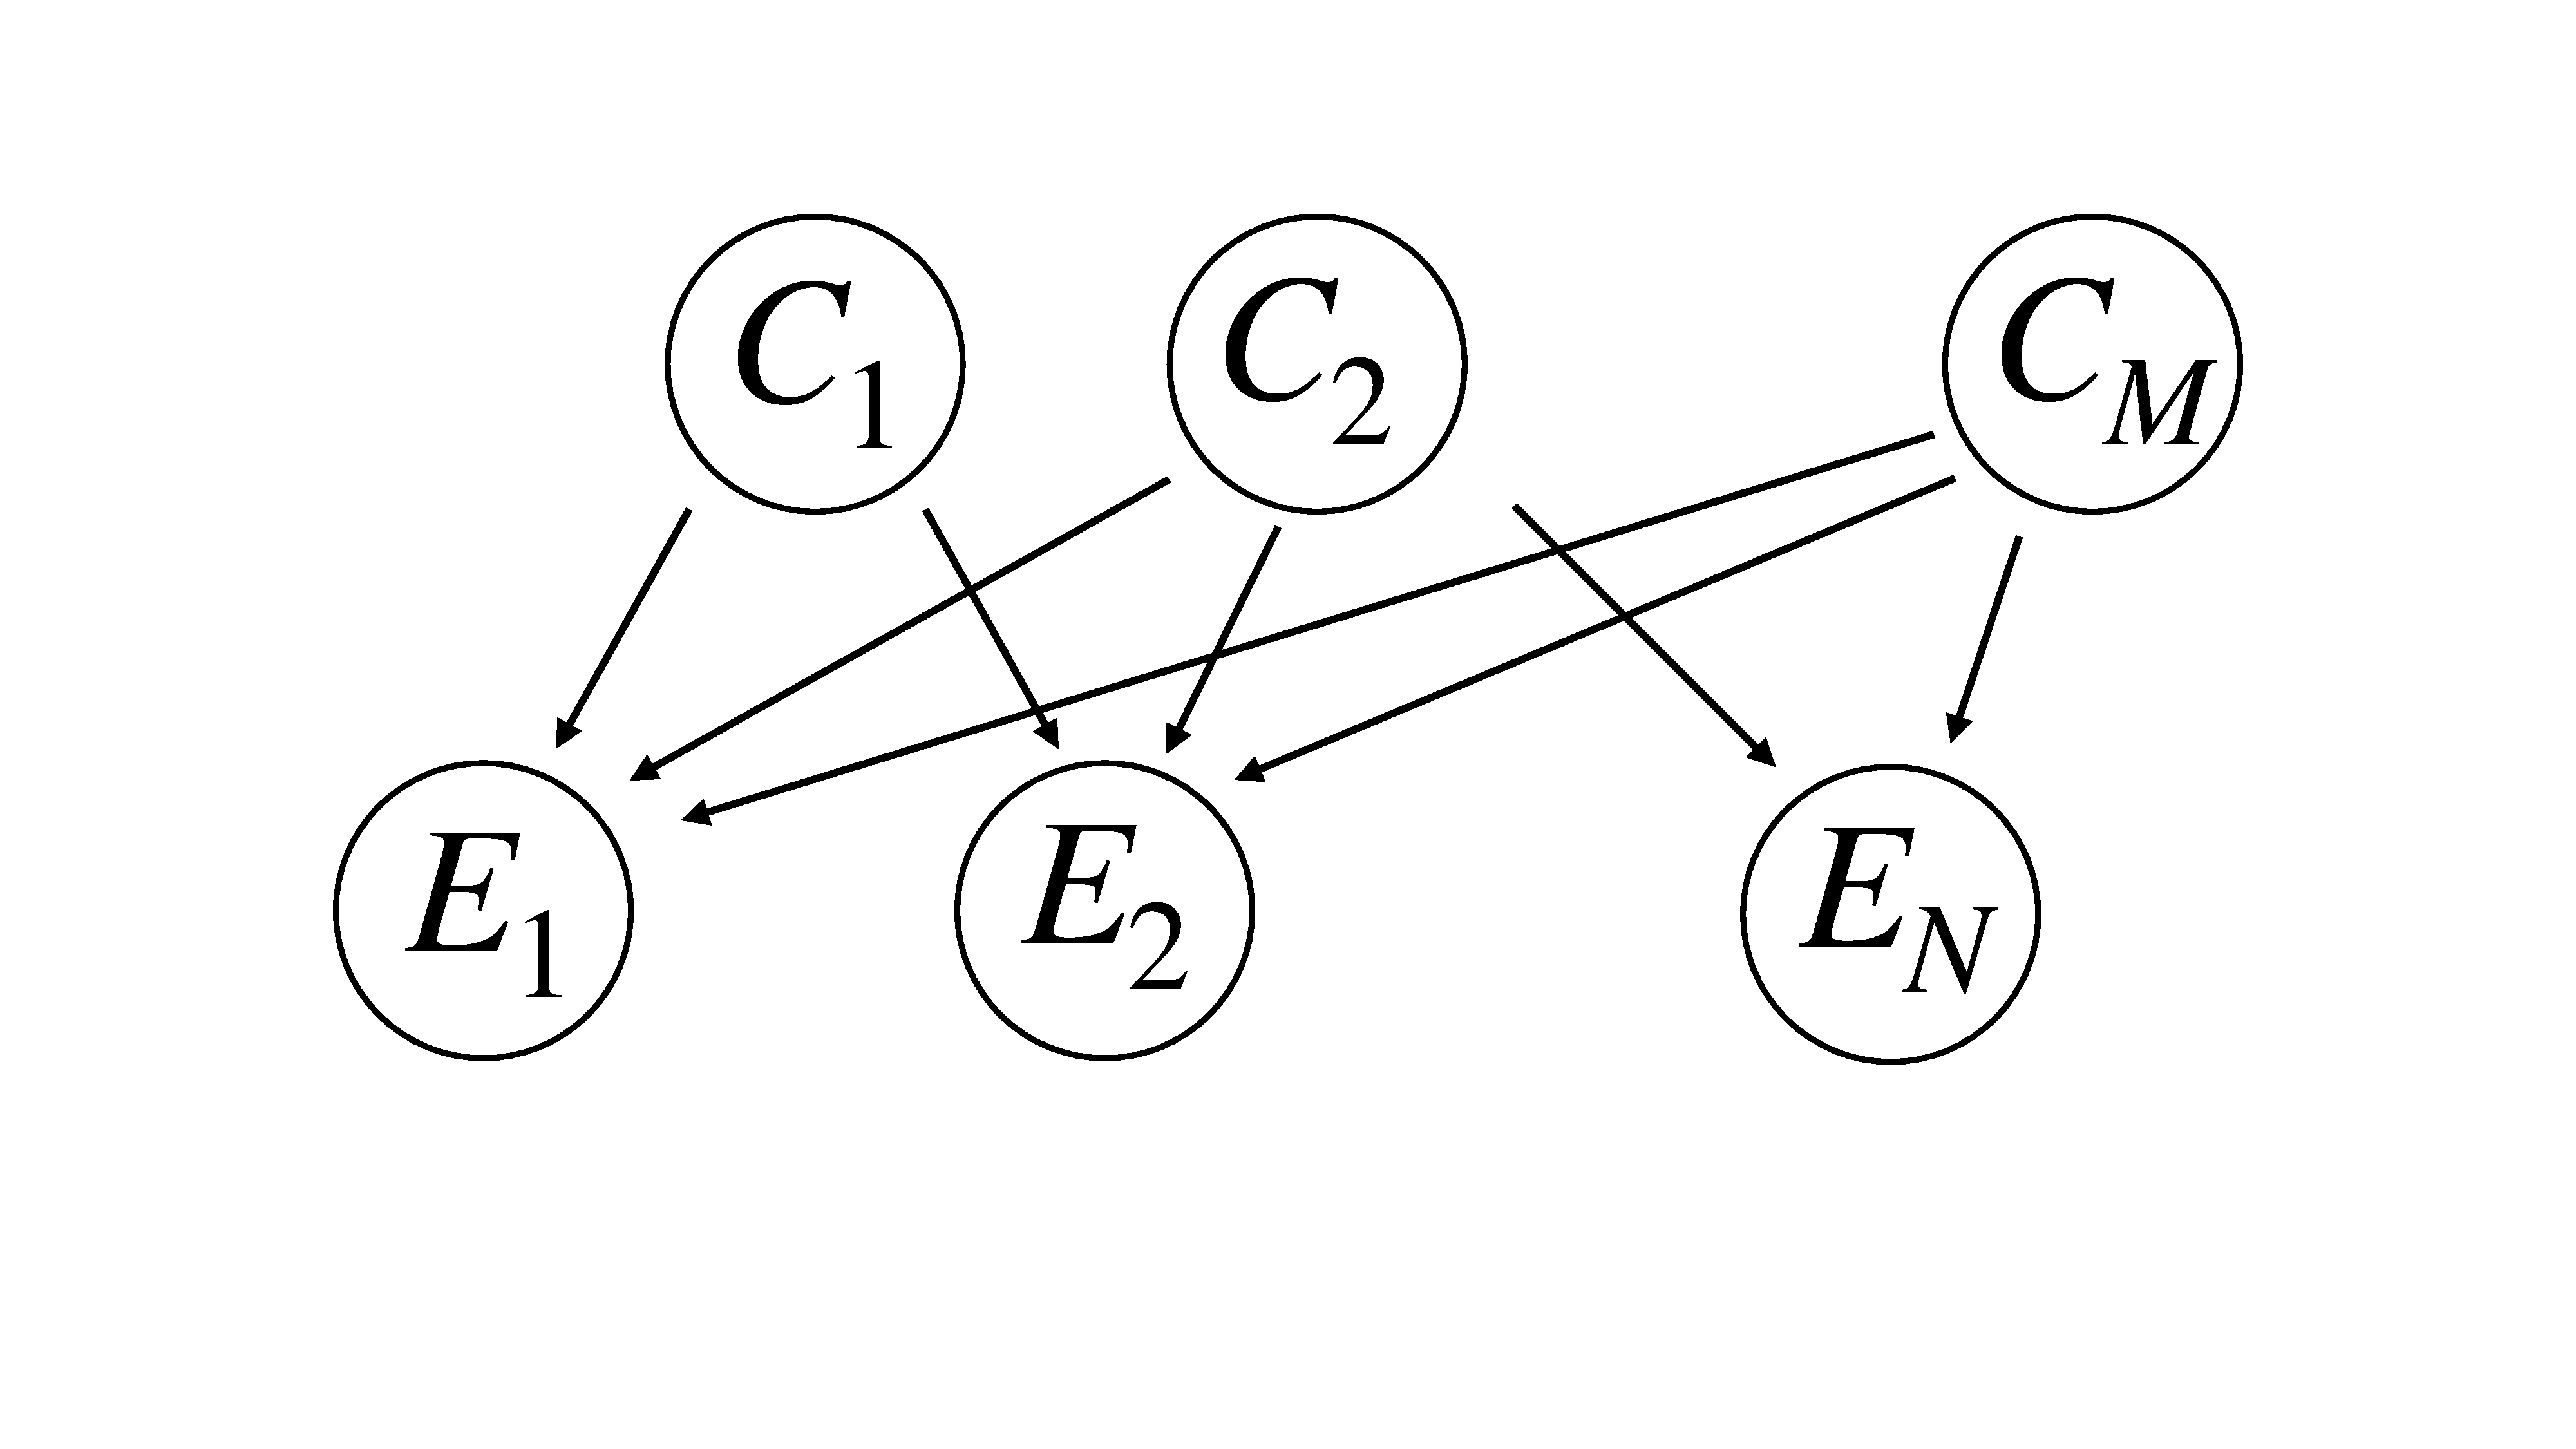
\includegraphics[page = 1, width=0.95\textwidth]{./figures/graphical_model}
\caption{Graphical model of causes and effects. Each arrow represents a probabilistic link}
\label{fig:graph_model}
\end{figure}
%------------------------------------------------------------
%
Borrowing the language of graphical models, the problem can be described by the Bayesian network of Fig.~\ref{fig:graph_model}, $C_{i}$ being the true number of events in each cause bin, given that we observe $E_{j}$ events per bin.
It's important to notice that as the links between cause and effect is probabilistic, so will be the number of true events per bin. Concretely,  given causes $C_i$ and effects $E_j$, we wish to estimate the conditional distribution
%
\begin{align}\label{eq:unf}
P(C_i | E_j)
\end{align}
%
Following standard Bayesian inference, Eq.~\ref{eq:unf} may be computed as
%
\begin{align}\label{eq:bayes_inf}
P(C_i | E_j) = \frac{P(E_j | C_i) P(C_i)}{\sum_{l=1}^{n_E} P(E_j| C_l) P(C_l)},
\end{align}
Eq.~\ref{eq:bayes_inf} is nothing other than Bayes' theorem stating that the posterior is proportional to the likelihood, provided that we multiply by the prior
%
\begin{align}
P(C_i | E_j) \propto P(E_j | C_i) P(C_i),
\end{align}
%
and the denominator is a normalization factor.
%The main issue in the practical application of Eq.~\ref{eq:bayes_inf} is that there is no closed to compute 
The unfolding algorithm proceeds as follows:
\begin{itemize}
\item
compute the number of expected events in bin $C_i$ given that $n(E_i)$ is the observed counting bin $E_j$\\
\begin{align}
n(C_i)|_{n(E_j)} = P(C_i | E_j) n(E_j);
\end{align}
\item
include effects from all observations\\
\begin{align}
n(C_i) = \sum_j P(C_i | E_j) n(E_j);
\end{align}
\item
correct for the effect of different efficiencies $\epsilon_i$\\
\begin{align}
\tilde{n}(C_i) = \frac{1}{\epsilon_i} n(C_i) = \frac{1}{\epsilon_i}\sum_{j=1}^{n_E} P(C_i | E_j) n(E_j);
\end{align}
with the efficiencies computed from the smearing matrix as
\begin{align}
\epsilon_i = \sum_{j=1}^{n_E} P(E_j | C_i) = \sum_{j=1}^{n_E} \lambda_{ij},
\end{align}
where $\lambda_{ij} = P(E_j | C_i)$ are the entries of a smearing matrix $\Lambda$ estimated from Monte Carlo simulations. 

The above algorithm is essentially the first form of Bayesian unfolding presented in Ref.~\cite{DAgostini:1994fjx}. Ref.~\cite{dagostini2010improved} introduced several improvements over the first version, like the explicit modelling of the smearing matrix and the inclusion its uncertainty as
%
\begin{align}
P(C_i | E_j) \longrightarrow P(C_i | E_j, \Lambda); \qquad P(C_i | E_j) = \int P(C_i | E_j) f(\Lambda) d\Lambda,
\end{align}
%
i.e. the posterior over causes depends explicitly on the smearing matrix $\Lambda$, which is sampled from a distribution $f(\Lambda)$.
Most notably, however, is the additional iteration of the algorithm. Bayesian inference only makes sense when we have a prior belief of what the possible values of the unobserved parameters are. Choosing a "correct" prior is a tricky task, as this choice, which is arbitrary, affects the posterior distribution.
Ref.~\cite{dagostini2010improved} suggests that the dependence on the prior can be reduced by iterating the unfolding procedure, by using the result of unfolding step $n$ as the prior of unfolding $n+1$.

We conclude the introduction with a brief discussions of the limitations of iterated Bayesian unfolding, and equivalent methods. The first obvious limitation is that the method relies on binning measurements into histograms. Binning can be problematic as aside with the exception of few limited case there's no obvious best binning, and each individual observable typically requires an ad hoc manual choice of the binning. Directly related to this is the fact that the total number of bins grows exponentially with the number of dimensions, each being a different observable. This means that differential cross section measurements beyond a few dimensions are impractical.

\end{itemize}
